% Options for packages loaded elsewhere
\PassOptionsToPackage{unicode}{hyperref}
\PassOptionsToPackage{hyphens}{url}
\PassOptionsToPackage{dvipsnames,svgnames,x11names}{xcolor}
%
\documentclass[
  letterpaper,
  DIV=11,
  numbers=noendperiod]{scrartcl}

\usepackage{amsmath,amssymb}
\usepackage{iftex}
\ifPDFTeX
  \usepackage[T1]{fontenc}
  \usepackage[utf8]{inputenc}
  \usepackage{textcomp} % provide euro and other symbols
\else % if luatex or xetex
  \usepackage{unicode-math}
  \defaultfontfeatures{Scale=MatchLowercase}
  \defaultfontfeatures[\rmfamily]{Ligatures=TeX,Scale=1}
\fi
\usepackage{lmodern}
\ifPDFTeX\else  
    % xetex/luatex font selection
\fi
% Use upquote if available, for straight quotes in verbatim environments
\IfFileExists{upquote.sty}{\usepackage{upquote}}{}
\IfFileExists{microtype.sty}{% use microtype if available
  \usepackage[]{microtype}
  \UseMicrotypeSet[protrusion]{basicmath} % disable protrusion for tt fonts
}{}
\makeatletter
\@ifundefined{KOMAClassName}{% if non-KOMA class
  \IfFileExists{parskip.sty}{%
    \usepackage{parskip}
  }{% else
    \setlength{\parindent}{0pt}
    \setlength{\parskip}{6pt plus 2pt minus 1pt}}
}{% if KOMA class
  \KOMAoptions{parskip=half}}
\makeatother
\usepackage{xcolor}
\usepackage{svg}
\setlength{\emergencystretch}{3em} % prevent overfull lines
\setcounter{secnumdepth}{-\maxdimen} % remove section numbering
% Make \paragraph and \subparagraph free-standing
\ifx\paragraph\undefined\else
  \let\oldparagraph\paragraph
  \renewcommand{\paragraph}[1]{\oldparagraph{#1}\mbox{}}
\fi
\ifx\subparagraph\undefined\else
  \let\oldsubparagraph\subparagraph
  \renewcommand{\subparagraph}[1]{\oldsubparagraph{#1}\mbox{}}
\fi

\usepackage{color}
\usepackage{fancyvrb}
\newcommand{\VerbBar}{|}
\newcommand{\VERB}{\Verb[commandchars=\\\{\}]}
\DefineVerbatimEnvironment{Highlighting}{Verbatim}{commandchars=\\\{\}}
% Add ',fontsize=\small' for more characters per line
\usepackage{framed}
\definecolor{shadecolor}{RGB}{241,243,245}
\newenvironment{Shaded}{\begin{snugshade}}{\end{snugshade}}
\newcommand{\AlertTok}[1]{\textcolor[rgb]{0.68,0.00,0.00}{#1}}
\newcommand{\AnnotationTok}[1]{\textcolor[rgb]{0.37,0.37,0.37}{#1}}
\newcommand{\AttributeTok}[1]{\textcolor[rgb]{0.40,0.45,0.13}{#1}}
\newcommand{\BaseNTok}[1]{\textcolor[rgb]{0.68,0.00,0.00}{#1}}
\newcommand{\BuiltInTok}[1]{\textcolor[rgb]{0.00,0.23,0.31}{#1}}
\newcommand{\CharTok}[1]{\textcolor[rgb]{0.13,0.47,0.30}{#1}}
\newcommand{\CommentTok}[1]{\textcolor[rgb]{0.37,0.37,0.37}{#1}}
\newcommand{\CommentVarTok}[1]{\textcolor[rgb]{0.37,0.37,0.37}{\textit{#1}}}
\newcommand{\ConstantTok}[1]{\textcolor[rgb]{0.56,0.35,0.01}{#1}}
\newcommand{\ControlFlowTok}[1]{\textcolor[rgb]{0.00,0.23,0.31}{#1}}
\newcommand{\DataTypeTok}[1]{\textcolor[rgb]{0.68,0.00,0.00}{#1}}
\newcommand{\DecValTok}[1]{\textcolor[rgb]{0.68,0.00,0.00}{#1}}
\newcommand{\DocumentationTok}[1]{\textcolor[rgb]{0.37,0.37,0.37}{\textit{#1}}}
\newcommand{\ErrorTok}[1]{\textcolor[rgb]{0.68,0.00,0.00}{#1}}
\newcommand{\ExtensionTok}[1]{\textcolor[rgb]{0.00,0.23,0.31}{#1}}
\newcommand{\FloatTok}[1]{\textcolor[rgb]{0.68,0.00,0.00}{#1}}
\newcommand{\FunctionTok}[1]{\textcolor[rgb]{0.28,0.35,0.67}{#1}}
\newcommand{\ImportTok}[1]{\textcolor[rgb]{0.00,0.46,0.62}{#1}}
\newcommand{\InformationTok}[1]{\textcolor[rgb]{0.37,0.37,0.37}{#1}}
\newcommand{\KeywordTok}[1]{\textcolor[rgb]{0.00,0.23,0.31}{#1}}
\newcommand{\NormalTok}[1]{\textcolor[rgb]{0.00,0.23,0.31}{#1}}
\newcommand{\OperatorTok}[1]{\textcolor[rgb]{0.37,0.37,0.37}{#1}}
\newcommand{\OtherTok}[1]{\textcolor[rgb]{0.00,0.23,0.31}{#1}}
\newcommand{\PreprocessorTok}[1]{\textcolor[rgb]{0.68,0.00,0.00}{#1}}
\newcommand{\RegionMarkerTok}[1]{\textcolor[rgb]{0.00,0.23,0.31}{#1}}
\newcommand{\SpecialCharTok}[1]{\textcolor[rgb]{0.37,0.37,0.37}{#1}}
\newcommand{\SpecialStringTok}[1]{\textcolor[rgb]{0.13,0.47,0.30}{#1}}
\newcommand{\StringTok}[1]{\textcolor[rgb]{0.13,0.47,0.30}{#1}}
\newcommand{\VariableTok}[1]{\textcolor[rgb]{0.07,0.07,0.07}{#1}}
\newcommand{\VerbatimStringTok}[1]{\textcolor[rgb]{0.13,0.47,0.30}{#1}}
\newcommand{\WarningTok}[1]{\textcolor[rgb]{0.37,0.37,0.37}{\textit{#1}}}

\providecommand{\tightlist}{%
  \setlength{\itemsep}{0pt}\setlength{\parskip}{0pt}}\usepackage{longtable,booktabs,array}
\usepackage{calc} % for calculating minipage widths
% Correct order of tables after \paragraph or \subparagraph
\usepackage{etoolbox}
\makeatletter
\patchcmd\longtable{\par}{\if@noskipsec\mbox{}\fi\par}{}{}
\makeatother
% Allow footnotes in longtable head/foot
\IfFileExists{footnotehyper.sty}{\usepackage{footnotehyper}}{\usepackage{footnote}}
\makesavenoteenv{longtable}
\usepackage{graphicx}
\makeatletter
\def\maxwidth{\ifdim\Gin@nat@width>\linewidth\linewidth\else\Gin@nat@width\fi}
\def\maxheight{\ifdim\Gin@nat@height>\textheight\textheight\else\Gin@nat@height\fi}
\makeatother
% Scale images if necessary, so that they will not overflow the page
% margins by default, and it is still possible to overwrite the defaults
% using explicit options in \includegraphics[width, height, ...]{}
\setkeys{Gin}{width=\maxwidth,height=\maxheight,keepaspectratio}
% Set default figure placement to htbp
\makeatletter
\def\fps@figure{htbp}
\makeatother

\KOMAoption{captions}{tableheading}
\makeatletter
\makeatother
\makeatletter
\makeatother
\makeatletter
\@ifpackageloaded{caption}{}{\usepackage{caption}}
\AtBeginDocument{%
\ifdefined\contentsname
  \renewcommand*\contentsname{Table of contents}
\else
  \newcommand\contentsname{Table of contents}
\fi
\ifdefined\listfigurename
  \renewcommand*\listfigurename{List of Figures}
\else
  \newcommand\listfigurename{List of Figures}
\fi
\ifdefined\listtablename
  \renewcommand*\listtablename{List of Tables}
\else
  \newcommand\listtablename{List of Tables}
\fi
\ifdefined\figurename
  \renewcommand*\figurename{Figure}
\else
  \newcommand\figurename{Figure}
\fi
\ifdefined\tablename
  \renewcommand*\tablename{Table}
\else
  \newcommand\tablename{Table}
\fi
}
\@ifpackageloaded{float}{}{\usepackage{float}}
\floatstyle{ruled}
\@ifundefined{c@chapter}{\newfloat{codelisting}{h}{lop}}{\newfloat{codelisting}{h}{lop}[chapter]}
\floatname{codelisting}{Listing}
\newcommand*\listoflistings{\listof{codelisting}{List of Listings}}
\makeatother
\makeatletter
\@ifpackageloaded{caption}{}{\usepackage{caption}}
\@ifpackageloaded{subcaption}{}{\usepackage{subcaption}}
\makeatother
\makeatletter
\@ifpackageloaded{tcolorbox}{}{\usepackage[skins,breakable]{tcolorbox}}
\makeatother
\makeatletter
\@ifundefined{shadecolor}{\definecolor{shadecolor}{rgb}{.97, .97, .97}}
\makeatother
\makeatletter
\makeatother
\makeatletter
\makeatother
\ifLuaTeX
  \usepackage{selnolig}  % disable illegal ligatures
\fi
\IfFileExists{bookmark.sty}{\usepackage{bookmark}}{\usepackage{hyperref}}
\IfFileExists{xurl.sty}{\usepackage{xurl}}{} % add URL line breaks if available
\urlstyle{same} % disable monospaced font for URLs
\hypersetup{
  pdftitle={Coup-Proofing via Capital Relocation},
  colorlinks=true,
  linkcolor={blue},
  filecolor={Maroon},
  citecolor={Blue},
  urlcolor={Blue},
  pdfcreator={LaTeX via pandoc}}

\title{Coup-Proofing via Capital Relocation}
\usepackage{etoolbox}
\makeatletter
\providecommand{\subtitle}[1]{% add subtitle to \maketitle
  \apptocmd{\@title}{\par {\large #1 \par}}{}{}
}
\makeatother
\subtitle{DSAN 6750 / PPOL 6805: GIS for Spatial Data Science}
\author{Jeff Jacobs}
\date{}

\begin{document}
\maketitle
\ifdefined\Shaded\renewenvironment{Shaded}{\begin{tcolorbox}[sharp corners, enhanced, breakable, boxrule=0pt, borderline west={3pt}{0pt}{shadecolor}, interior hidden, frame hidden]}{\end{tcolorbox}}\fi

\hypertarget{introduction}{%
\subsection{Introduction}\label{introduction}}

Several previous studies have found robust relationships between spatial
properties of a country's \textbf{capital city} and that country's
propensity for \textbf{conflict} and \textbf{misgovernance}.

Perceptions of this linkage also have an effect on ``coup-proofing''
decisions made by national governments. A recent BBC interview with
Equatorial Guinea's President Teodoro Obiang, for example, highlighted
this as a factor behind his decision to relocate the capital city:

\begin{quote}
It's the remoteness of Oyala that makes it so appealing to President
Obiang. In a rare interview he described how rebels had recently plotted
a seaborne assault on his palace in the current capital, Malabo. `We
need a secure place for my government and for future governments. That's
why we have created Oyala, to guarantee the government of Equatorial
Guinea.' {[}@sackur\_equatorial\_2012{]}
\end{quote}

This case is far from exceptional, as an even more recent
\emph{Washington Post} article points out with respect to Myanmar's
decision to move its capital from Yangon to Naypyidaw:

\begin{quote}
Analysts have described the decision as motivated by a desire to secure
the military's seat of power from any threat of protests or invasions.
{[}@berger\_myanmars\_2021{]}
\end{quote}

Most of these studies, however, are based on observations of
\textbf{conflict events}. In this study, we study the more fundamental
variable of a capital's distance from the \textbf{population centroid}
of the country.

\hypertarget{literature-review}{%
\subsection{Literature Review}\label{literature-review}}

@campante\_capital\_2019 analyzes the relationship between the location
of a \textbf{capital city} and the degree of conflict and misgovernance
in a given country. Their two key findings are that:

\begin{quote}
Conflict is more likely to emerge (and dislodge incumbents) closer to
the capital
\end{quote}

and

\begin{quote}
Isolated capitals are associated with misgovernance.
\end{quote}

This first finding is illustrated in \textbf{?@fig-conflict-dist}

\includesvg{images/conflict_dist.svg}

\hypertarget{methodology}{%
\subsection{Methodology}\label{methodology}}

The \textbf{population centroids} we use herein might require some
explanation, since the term ``centroid'' can be ambiguous.

Here, the population centroids are drawn from @hall\_population\_2019

\hypertarget{exploratory-data-analysis-eda}{%
\subsection{Exploratory Data Analysis
(EDA)}\label{exploratory-data-analysis-eda}}

Here we plot the base GIS objects we're analyzing: the location of each
\textbf{capital city} (in purple) and each \textbf{population centroid}
(in yellow).

\begin{Shaded}
\begin{Highlighting}[]
\FunctionTok{library}\NormalTok{(tidyverse) }\SpecialCharTok{|\textgreater{}} \FunctionTok{suppressPackageStartupMessages}\NormalTok{()}
\FunctionTok{library}\NormalTok{(sf) }\SpecialCharTok{|\textgreater{}} \FunctionTok{suppressPackageStartupMessages}\NormalTok{()}
\FunctionTok{library}\NormalTok{(mapview) }\SpecialCharTok{|\textgreater{}} \FunctionTok{suppressPackageStartupMessages}\NormalTok{()}
\FunctionTok{library}\NormalTok{(units) }\SpecialCharTok{|\textgreater{}} \FunctionTok{suppressPackageStartupMessages}\NormalTok{()}
\NormalTok{cb\_palette }\OtherTok{\textless{}{-}} \FunctionTok{c}\NormalTok{(}\StringTok{"\#E69F00"}\NormalTok{, }\StringTok{"\#56B4E9"}\NormalTok{, }\StringTok{"\#009E73"}\NormalTok{, }\StringTok{"\#F0E442"}\NormalTok{, }\StringTok{"\#0072B2"}\NormalTok{, }\StringTok{"\#D55E00"}\NormalTok{, }\StringTok{"\#CC79A7"}\NormalTok{)}
\end{Highlighting}
\end{Shaded}

\begin{Shaded}
\begin{Highlighting}[]
\NormalTok{merged\_long\_sf }\OtherTok{\textless{}{-}} \FunctionTok{readRDS}\NormalTok{(}\StringTok{"merged\_long\_sf.rds"}\NormalTok{)}
\FunctionTok{mapview}\NormalTok{(merged\_long\_sf, }\AttributeTok{zcol=}\StringTok{"name"}\NormalTok{, }\AttributeTok{cex=}\DecValTok{4}\NormalTok{, }\AttributeTok{label=}\StringTok{"geounit"}\NormalTok{)}
\end{Highlighting}
\end{Shaded}

\begin{verbatim}
Warning in validateCoords(lng, lat, funcName): Data contains 3 rows with either
missing or invalid lat/lon values and will be ignored
\end{verbatim}

\begin{figure}[H]

{\centering 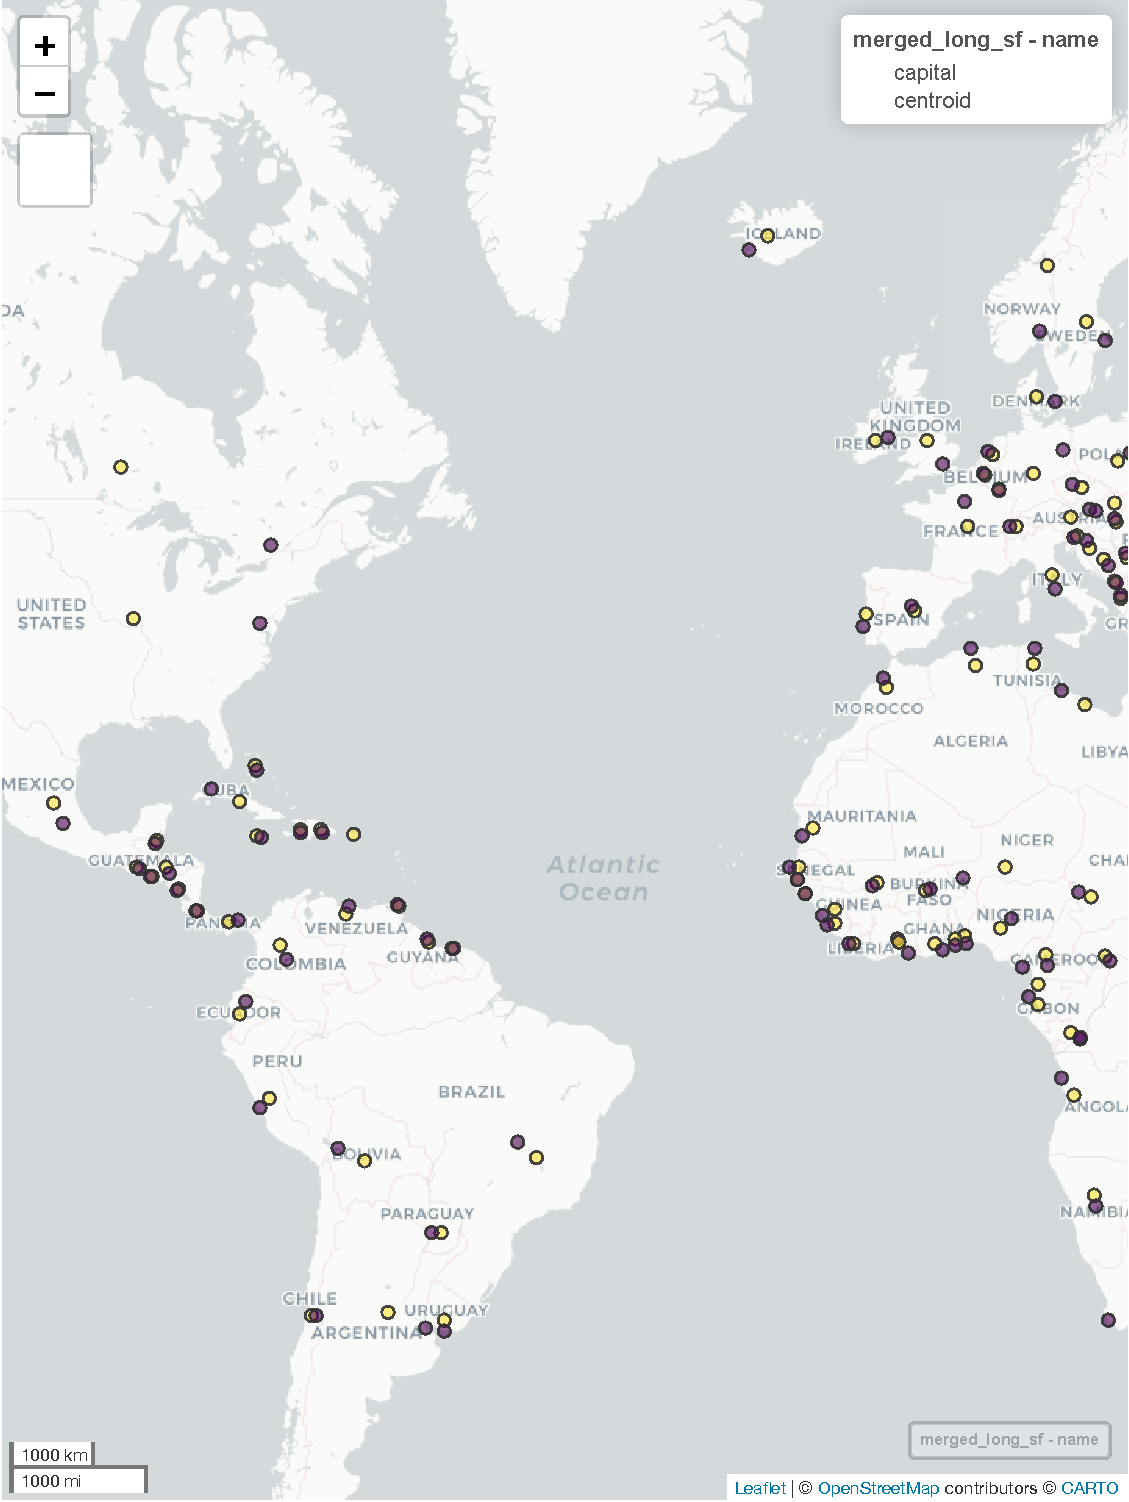
\includegraphics{index_files/figure-pdf/load-eda-1.pdf}

}

\end{figure}

We then construct an \textbf{area-normalized} measure of
capital-centroid distance \(\text{dist}^{\textsf{AN}}\), using the
formula

\[
\text{dist}^{\textsf{AN}}_i = \text{dist}_i / \sqrt{\text{area}_i}.
\]

A plot of this measure by country looks as follows:

\begin{Shaded}
\begin{Highlighting}[]
\NormalTok{merged\_area\_sf }\OtherTok{\textless{}{-}} \FunctionTok{readRDS}\NormalTok{(}\StringTok{"merged\_area\_sf.rds"}\NormalTok{)}
\FunctionTok{mapview}\NormalTok{(merged\_area\_sf, }\AttributeTok{zcol=}\StringTok{"scaled\_dist"}\NormalTok{)}
\end{Highlighting}
\end{Shaded}

\begin{figure}[H]

{\centering 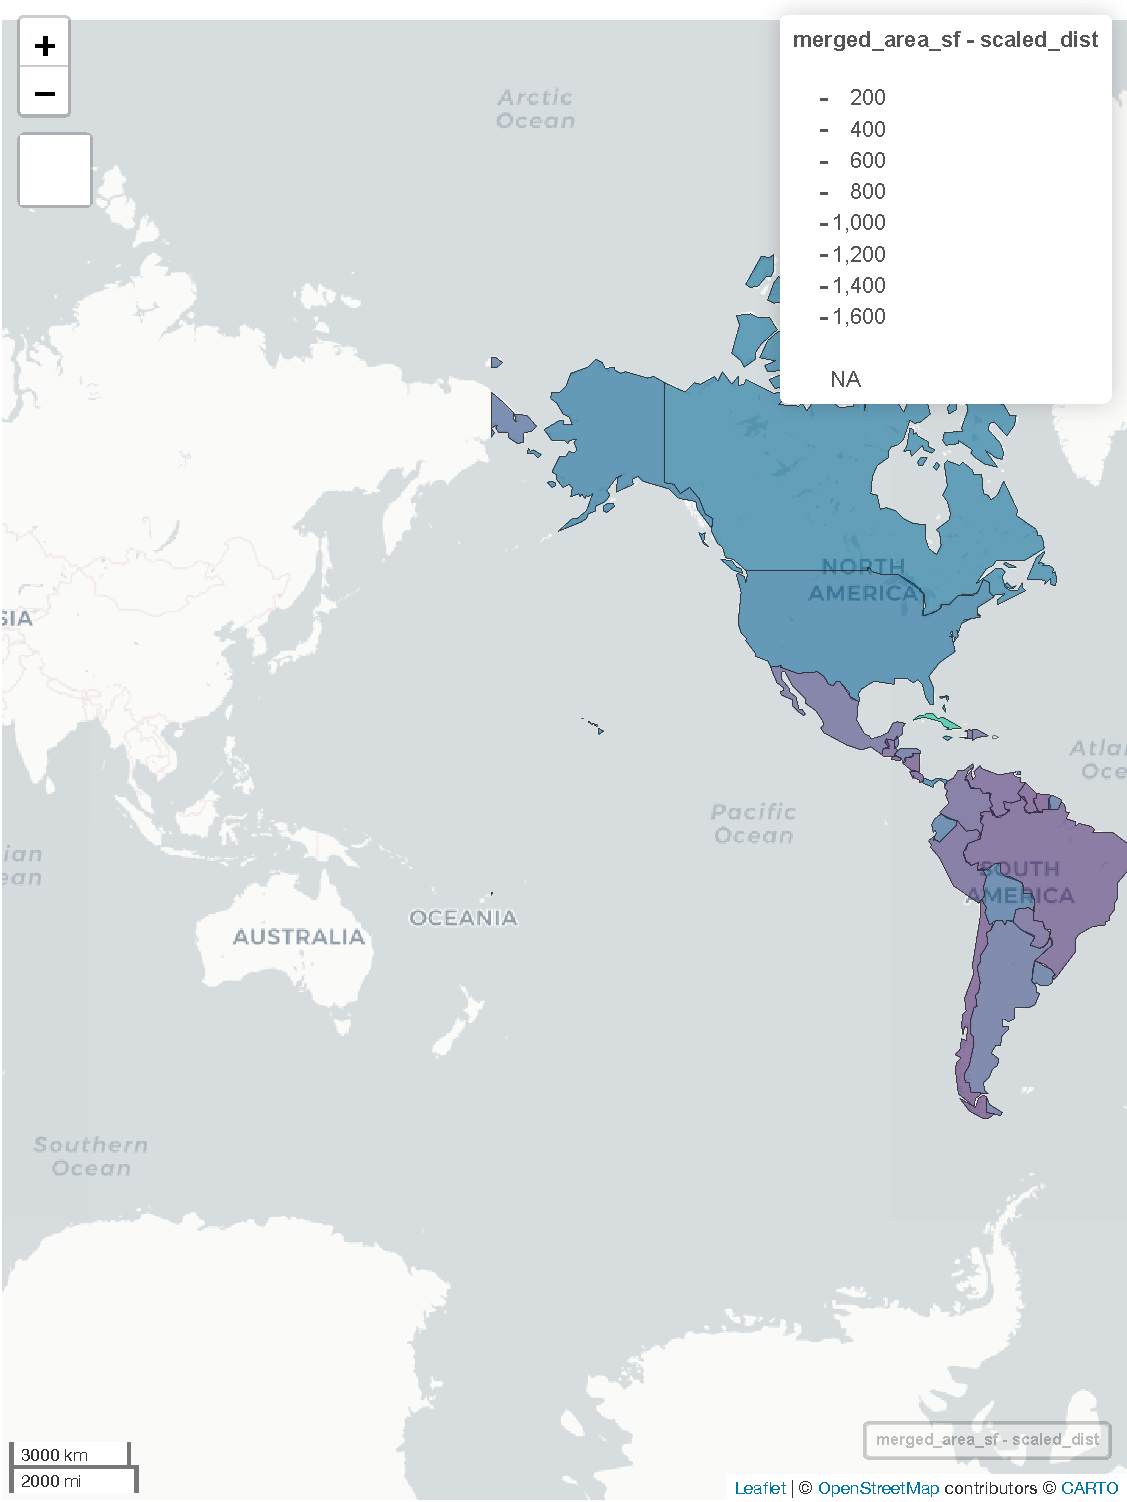
\includegraphics{index_files/figure-pdf/plot-area-1.pdf}

}

\end{figure}

\hypertarget{hypothesis-testing-regression}{%
\subsection{Hypothesis Testing
(Regression)}\label{hypothesis-testing-regression}}

\begin{Shaded}
\begin{Highlighting}[]
\NormalTok{merged\_sub\_sf }\OtherTok{\textless{}{-}} \FunctionTok{readRDS}\NormalTok{(}\StringTok{"merged\_sub\_sf.rds"}\NormalTok{)}
\NormalTok{merged\_sub\_sf }\SpecialCharTok{|\textgreater{}} \FunctionTok{head}\NormalTok{()}
\end{Highlighting}
\end{Shaded}

\begin{longtable}[]{@{}
  >{\raggedright\arraybackslash}p{(\columnwidth - 26\tabcolsep) * \real{0.1126}}
  >{\raggedright\arraybackslash}p{(\columnwidth - 26\tabcolsep) * \real{0.0315}}
  >{\raggedleft\arraybackslash}p{(\columnwidth - 26\tabcolsep) * \real{0.0405}}
  >{\raggedleft\arraybackslash}p{(\columnwidth - 26\tabcolsep) * \real{0.0225}}
  >{\raggedright\arraybackslash}p{(\columnwidth - 26\tabcolsep) * \real{0.0766}}
  >{\raggedleft\arraybackslash}p{(\columnwidth - 26\tabcolsep) * \real{0.0405}}
  >{\raggedright\arraybackslash}p{(\columnwidth - 26\tabcolsep) * \real{0.0811}}
  >{\raggedleft\arraybackslash}p{(\columnwidth - 26\tabcolsep) * \real{0.0631}}
  >{\raggedleft\arraybackslash}p{(\columnwidth - 26\tabcolsep) * \real{0.0360}}
  >{\raggedleft\arraybackslash}p{(\columnwidth - 26\tabcolsep) * \real{0.0586}}
  >{\raggedleft\arraybackslash}p{(\columnwidth - 26\tabcolsep) * \real{0.0541}}
  >{\raggedright\arraybackslash}p{(\columnwidth - 26\tabcolsep) * \real{0.1396}}
  >{\raggedright\arraybackslash}p{(\columnwidth - 26\tabcolsep) * \real{0.1216}}
  >{\raggedright\arraybackslash}p{(\columnwidth - 26\tabcolsep) * \real{0.1216}}@{}}
\toprule\noalign{}
\begin{minipage}[b]{\linewidth}\raggedright
geounit
\end{minipage} & \begin{minipage}[b]{\linewidth}\raggedright
iso\_a3
\end{minipage} & \begin{minipage}[b]{\linewidth}\raggedleft
OBJECTID
\end{minipage} & \begin{minipage}[b]{\linewidth}\raggedleft
ID\_0
\end{minipage} & \begin{minipage}[b]{\linewidth}\raggedright
NAME\_ENGLI
\end{minipage} & \begin{minipage}[b]{\linewidth}\raggedleft
OUT\_FLAG
\end{minipage} & \begin{minipage}[b]{\linewidth}\raggedright
NAME
\end{minipage} & \begin{minipage}[b]{\linewidth}\raggedleft
dist
\end{minipage} & \begin{minipage}[b]{\linewidth}\raggedleft
area
\end{minipage} & \begin{minipage}[b]{\linewidth}\raggedleft
scaled\_dist
\end{minipage} & \begin{minipage}[b]{\linewidth}\raggedleft
total\_score
\end{minipage} & \begin{minipage}[b]{\linewidth}\raggedright
geometry
\end{minipage} & \begin{minipage}[b]{\linewidth}\raggedright
centroid
\end{minipage} & \begin{minipage}[b]{\linewidth}\raggedright
capital
\end{minipage} \\
\midrule\noalign{}
\endhead
\bottomrule\noalign{}
\endlastfoot
Tanzania & TZA & 227 & 227 & Tanzania & 0 & Dar es Salaam & 324758.1
{[}m{]} & 885800 & 345.0580 {[}m{]} & 0.007 & MULTIPOLYGON (((33.90371
-0\ldots{} & POINT (36.5813 -5.612844) & POINT (39.2664 -6.798067) \\
Canada & CAN & 42 & 42 & Canada & 0 & Ottawa & 1410811.7 {[}m{]} &
8788700 & 475.8902 {[}m{]} & 0.001 & MULTIPOLYGON (((-122.84 49,\ldots{}
& POINT (-92.673 51.33108) & POINT (-75.70196 45.41864) \\
United States of America & USA & 244 & 244 & United States & 0 &
Washington, D.C. & 1227411.4 {[}m{]} & 9147420 & 405.8269 {[}m{]} &
0.022 & MULTIPOLYGON (((-122.84 49,\ldots{} & POINT (-91.24719 39.43566)
& POINT (-77.01136 38.9015) \\
Kazakhstan & KAZ & 117 & 117 & Kazakhstan & 0 & Nur-Sultan & 227074.6
{[}m{]} & 2699700 & 138.2009 {[}m{]} & 0.010 & MULTIPOLYGON (((87.35997
49\ldots{} & POINT (69.7252 49.45229) & POINT (71.42777 51.18113) \\
Uzbekistan & UZB & 246 & 246 & Uzbekistan & 0 & Tashkent & 168011.1
{[}m{]} & 440653 & 253.0985 {[}m{]} & 0.005 & MULTIPOLYGON (((55.96819
41\ldots{} & POINT (67.77264 40.30358) & POINT (69.26882 41.30383) \\
Papua New Guinea & PNG & 175 & 175 & Papua New Guinea & 0 & Port Moresby
& 289887.1 {[}m{]} & 452860 & 430.7714 {[}m{]} & 0.025 & MULTIPOLYGON
(((141.0002 -2\ldots{} & POINT (146.2921 -7.014699) & POINT (147.1925
-9.464708) \\
\end{longtable}

\begin{Shaded}
\begin{Highlighting}[]
\NormalTok{merged\_sub\_sf }\SpecialCharTok{|\textgreater{}} \FunctionTok{ggplot}\NormalTok{(}\FunctionTok{aes}\NormalTok{(}\AttributeTok{x=}\NormalTok{scaled\_dist, }\AttributeTok{y=}\NormalTok{total\_score, }\AttributeTok{label=}\NormalTok{NAME\_ENGLI)) }\SpecialCharTok{+}
  \FunctionTok{geom\_point}\NormalTok{() }\SpecialCharTok{+}
  \FunctionTok{geom\_smooth}\NormalTok{(}\AttributeTok{method=}\StringTok{\textquotesingle{}lm\textquotesingle{}}\NormalTok{, }\AttributeTok{formula=}\NormalTok{ y}\SpecialCharTok{\textasciitilde{}}\NormalTok{x) }\SpecialCharTok{+}
  \FunctionTok{geom\_text}\NormalTok{(}\AttributeTok{size=}\DecValTok{4}\NormalTok{, }\AttributeTok{nudge\_y =} \FloatTok{0.075}\NormalTok{) }\SpecialCharTok{+}
  \FunctionTok{theme\_classic}\NormalTok{()}
\end{Highlighting}
\end{Shaded}

\begin{verbatim}
Warning: The `scale_name` argument of `continuous_scale()` is deprecated as of ggplot2
3.5.0.
\end{verbatim}

\begin{verbatim}
Warning: Removed 4 rows containing non-finite outside the scale range
(`stat_smooth()`).
\end{verbatim}

\begin{verbatim}
Warning: The following aesthetics were dropped during statistical transformation: label.
i This can happen when ggplot fails to infer the correct grouping structure in
  the data.
i Did you forget to specify a `group` aesthetic or to convert a numerical
  variable into a factor?
\end{verbatim}

\begin{verbatim}
Warning: Removed 4 rows containing missing values or values outside the scale range
(`geom_point()`).
\end{verbatim}

\begin{verbatim}
Warning: Removed 4 rows containing missing values or values outside the scale range
(`geom_text()`).
\end{verbatim}

\begin{figure}[H]

{\centering 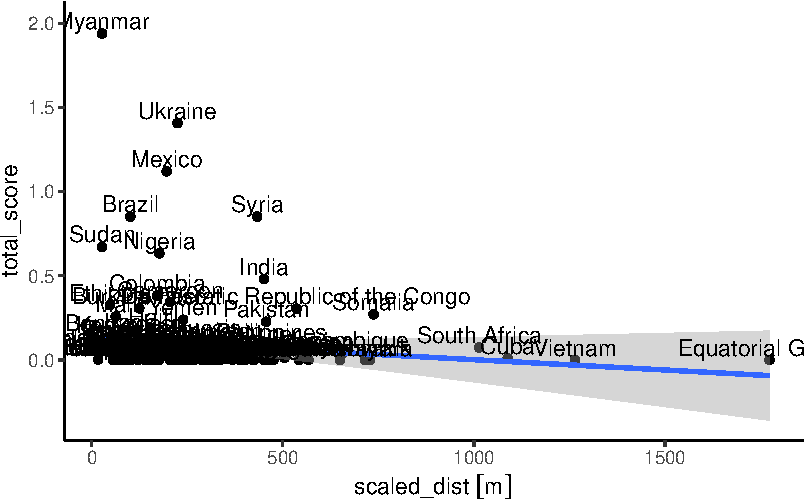
\includegraphics{index_files/figure-pdf/unnamed-chunk-5-1.pdf}

}

\end{figure}

\hypertarget{discussion}{%
\subsection{Discussion}\label{discussion}}

\hypertarget{conclusion}{%
\subsection{Conclusion}\label{conclusion}}

Our evidence indicates that the spatial dynamics of \textbf{conflict}
differ from the spatial dynamics of \textbf{misgovernance}. Whereas



\end{document}
